\hypertarget{interface_t_p_chart_pie}{
\section{TPChartPie Class Reference}
\label{interface_t_p_chart_pie}\index{TPChartPie@{TPChartPie}}
}
{\tt \#import $<$TPChartPie.h$>$}

Inheritance diagram for TPChartPie::\begin{figure}[H]
\begin{center}
\leavevmode
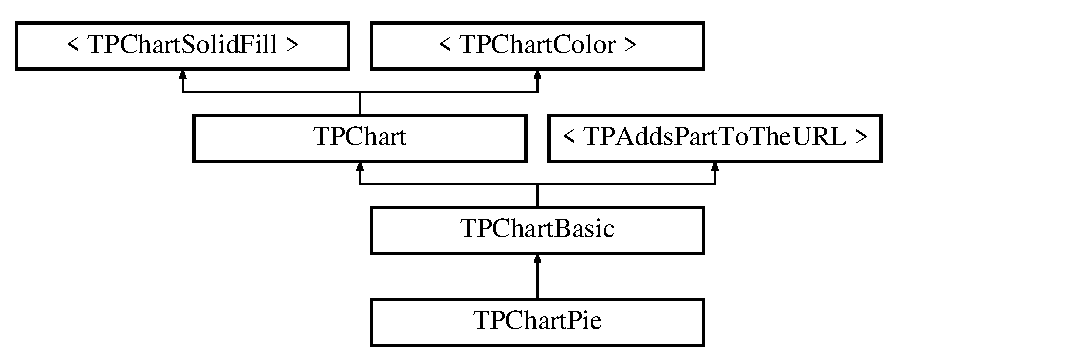
\includegraphics[height=4cm]{interface_t_p_chart_pie}
\end{center}
\end{figure}
\subsection*{Properties}
\begin{CompactItemize}
\item 
TPChartTypePie \hyperlink{interface_t_p_chart_pie_f9a2aea3325ac699501b0cbea394e0d7}{type}
\item 
float \hyperlink{interface_t_p_chart_pie_03ce748bdb6e02278b78963049dee536}{angle}
\end{CompactItemize}


\subsection{Detailed Description}
Pie Chart example: \href{http://chart.apis.google.com/chart?cht=p3&chd=s:Uf9a&chs=250x100&chl=January}{\tt http://chart.apis.google.com/chart?cht=p3\&chd=s:Uf9a\&chs=250x100\&chl=January}$|$February$|$March$|$April 

\subsection{Property Documentation}
\hypertarget{interface_t_p_chart_pie_03ce748bdb6e02278b78963049dee536}{
\index{TPChartPie@{TPChartPie}!angle@{angle}}
\index{angle@{angle}!TPChartPie@{TPChartPie}}
\subsubsection[{angle}]{\setlength{\rightskip}{0pt plus 5cm}- (float) angle\hspace{0.3cm}{\tt  \mbox{[}read, write, assign\mbox{]}}}}
\label{interface_t_p_chart_pie_03ce748bdb6e02278b78963049dee536}


Angle to rotate the chart in radians \hypertarget{interface_t_p_chart_pie_f9a2aea3325ac699501b0cbea394e0d7}{
\index{TPChartPie@{TPChartPie}!type@{type}}
\index{type@{type}!TPChartPie@{TPChartPie}}
\subsubsection[{type}]{\setlength{\rightskip}{0pt plus 5cm}- (TPChartTypePie) type\hspace{0.3cm}{\tt  \mbox{[}read, write, assign\mbox{]}}}}
\label{interface_t_p_chart_pie_f9a2aea3325ac699501b0cbea394e0d7}


Type of the Chart 2D = P 3D = p3 Centric = C 

The documentation for this class was generated from the following file:\begin{CompactItemize}
\item 
TPChartPie.h\end{CompactItemize}
